\section{\system: Mapping AWQ onto Edge Platforms}


AWQ can substantially reduce the size of LLMs. However, converting the theoretical memory savings from W4A16 (4-bit weight, 16-bit activation) quantization into measured speedup is non-trivial. Alternative W8A8 quantization methods, such as SmoothQuant~\cite{xiao2022smoothquant}, maintain \textit{the same} data precision for both storage and computation. This allows the dequantization procedure to be seamlessly integrated into the computation kernel's epilogue. On the other hand, W4A16 quantization employs \textit{different} data types for memory access and computation. As a result, its dequantization must be incorporated into the primary computation loop for optimal performance, posing implementation challenges. To tackle this, we introduce \system: a nimble system for AWQ model inference. It boasts a PyTorch frontend and a backend harnessing device-specific instruction sets (e.g., CUDA/PTX, Neon, AVX).

\subsection{Why AWQ Helps Accelerate On-Device LLMs}

\begin{figure*}
    \centering
     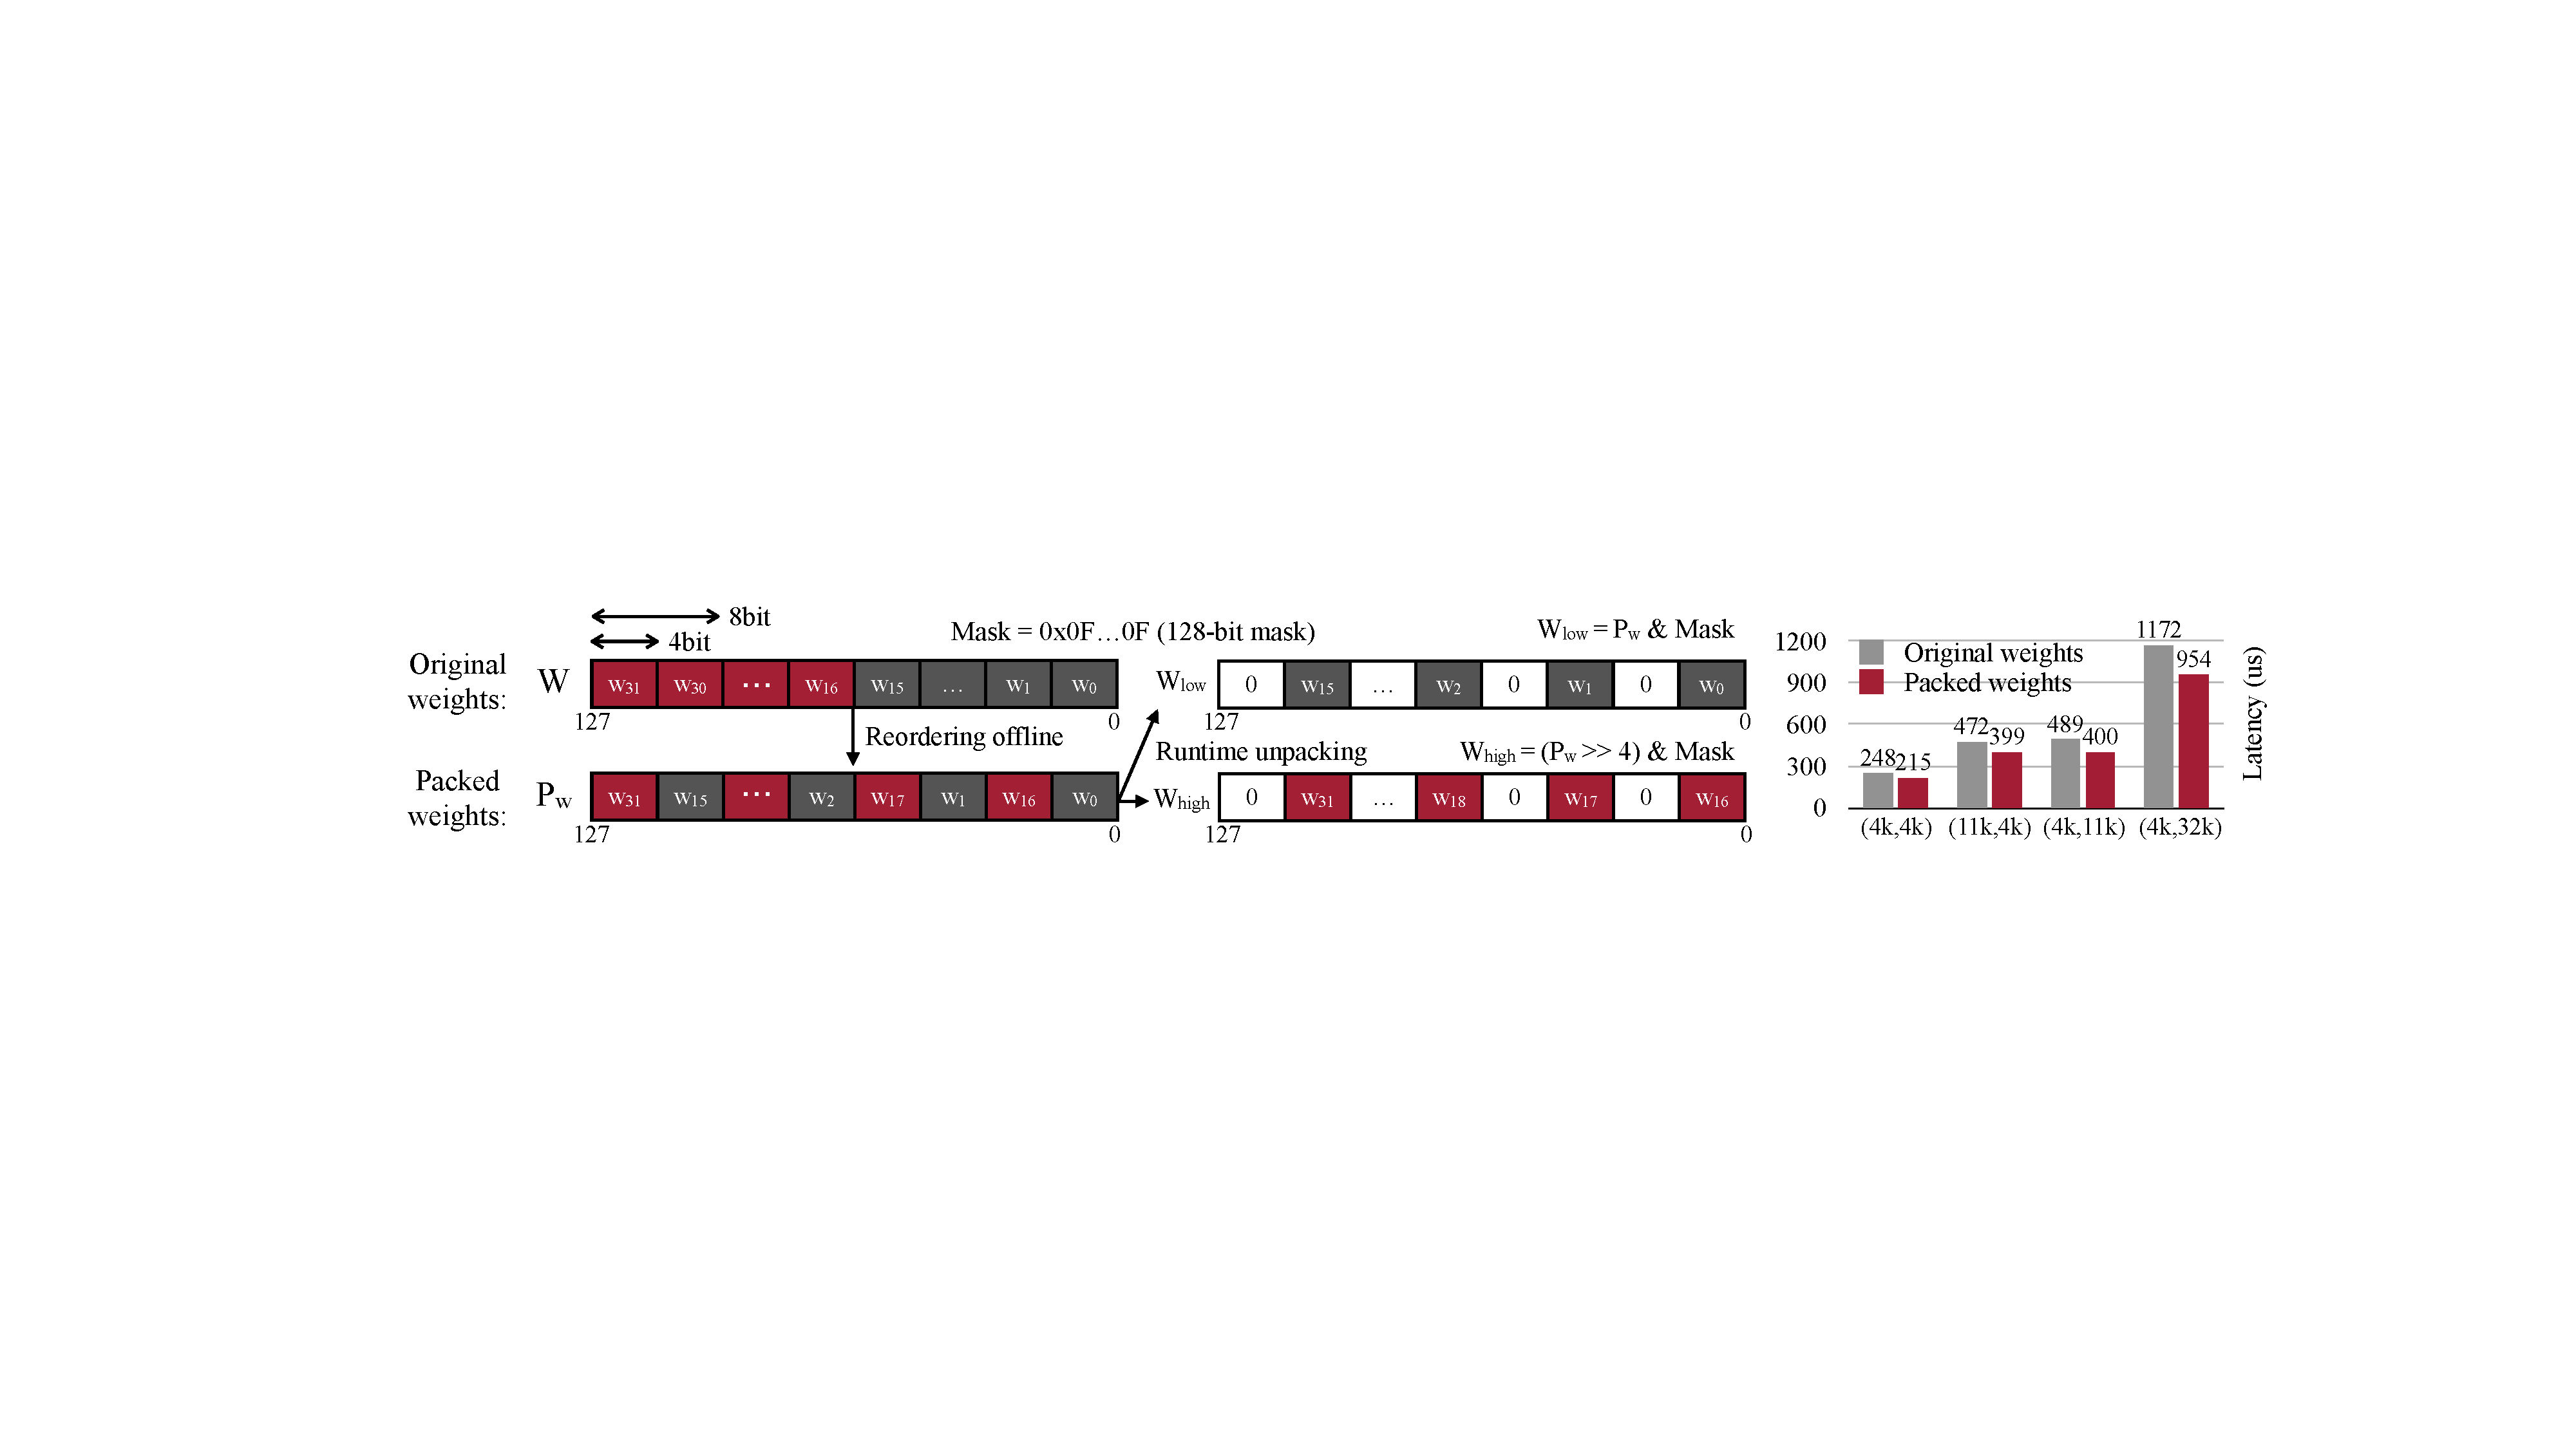
\includegraphics[width=\textwidth]{figures/weight_packing.pdf}
    \caption{SIMD-aware weight packing for ARM NEON with 128-bit SIMD units. Original weights are reordered and packed to align with the bit width so that the weights can be unpacked into bytes at runtime using AND and shift bitwise operations with a 128-bit mask.} %
    \label{fig:weight_packing}
\end{figure*}




To understand the acceleration opportunities in quantized LLMs on the edge, we start by profiling the latency breakdown of LLaMA-7B~\cite{touvron2023llama} model on an RTX 4090 GPU. We adopt an inference batch size of 1, catering for edge use cases, and implement the model in FP16 with NVIDIA FasterTransformer. 

\myparagraph{Context \textit{vs} generation latency.} As in Figure~\ref{fig:memory_bound_analysis}(a), it takes 310 ms to generate 20 tokens, while summarizing a prompt with 200 tokens only takes 10 ms. Consequently, the generation phase is substantially slower than the context stage, particularly for on-device interactive applications. 

\myparagraph{Generation stage is memory-bound.} To accelerate the generation phase, we conduct a roofline analysis in Figure~\ref{fig:memory_bound_analysis}(b). The 4090 GPU has a peak computation throughput of 165 TFLOPS and a memory bandwidth of 1TB/s. Therefore, any workload with arithmetic intensity (the ratio of FLOPs to memory access) less than 165 is  memory bounded on 4090 GPUs. Notably, when executed in FP16, the generation stage for on-device LLMs has arithmetic intensity$\approx$1. This underscores the memory-bound nature of the workload. Since the FLOPs of a given model is fixed, the only way to improve the peak performance is to reduce the total amount of memory traffic. AWQ reduces the weight memory by four times. 


\myparagraph{Weight access dominates memory traffic.}
 We therefore further break down the memory access for weight and activation in Figure~\ref{fig:memory_bound_analysis}(c). Clearly, weight access dominates the memory traffic for on-device LLMs. Quantizing the model weights to 4 bit integers will approximately increase the arithmetic intensity to 4 FLOPs/Byte, leading to a 4TFLOPS peak performance in Figure~\ref{fig:memory_bound_analysis}(b). Since weight-only quantization leads to a lower bit width for weights (and thus higher theoretical performance upper bound), it is natural for AWQ to follow this setting for on-device LLM applications.


\subsection{Deploy AWQ with \system}

To this end, we demonstrated that 4-bit weight quantization could lead to a 4$\times$ theoretical peak performance. We further design \system to realize this speedup. On GPUs, we only focus on implementing essential components, including attention, layer normalization, and linear projection kernels. The flexible frontend allows easy customization and fast support for new models. \system with 4-bit AWQ achieves more than \textbf{3$\times$} speedup compared with the Huggingface FP16 implementation across different families of LLMs on GPUs. On CPUs, we lower the entire computation graph to C++ to minimize overhead.

\myparagraph{On-the-fly weight dequantization.} For quantized layers, as the hardware does not provide multiplication instructions between INT4 and FP16, we need to dequantize the integers to FP16 before performing matrix computation. We avoid writing dequantized weights into DRAM by fusing dequantization kernels with the matrix multplication kernel. Note that such fusion is adopted for both matrix-matrix (MM) and matrix-vector (MV) product kernels. %


\myparagraph{SIMD-aware weight packing.} On-the-fly weight dequantization reduces intermediate DRAM access, but remains expensive. For instance, dequantizing \textit{a single 4-bit weight} involves 1 shift, 1 bitwise AND, and 1 FMA scaling operations, while the dequantized weight undergoes only 1 FMA computation. This process is particularly costly on CPUs with SIMD architecture that favor vectorized instructions. To mitigate this, we suggest platform-specific weight packing tailored to the bitwidth of a device's SIMD units. Figure~\ref{fig:weight_packing} demonstrates our strategy for ARM CPUs with 128-bit SIMD registers offering up to 1.2$\times$ speedup. Here, each register holds 32 4-bit weights, sequenced as $w_0, w_{16}, w_{1}, w_{17}, ..., w_{15}, w_{31}$. This approach requires just three SIMD instructions to unpack \textit{all 32 weights}, as opposed to 3 scalar instructions \textit{per weight} in a conventional packing ($w_0, w_1, ..., w_{31}$). Generally, for $2^n$-bit SIMD registers, adjacent weights will have indices off by $1/8\times2^n$, since each register can hold $1/8\times2^n$ 8-bit integers. On GPUs, we found it more efficient to pack each 8 weights into $w_{\{0,2,4,6,1,3,5,7\}}$ following~\cite{kim2022says}. 

\myparagraph{Kernel fusion.} We also extensively apply kernel fusion to optimize on-device LLM inference. For layer normalization, we fuse all operators (\eg multiplication, division and square root) into a single kernel. For attention layers, we fuse QKV projections into a single kernel, and also perform on-the-fly positional embedding calculation. We also pre-allocate KV caches and perform cache updates within the attention kernel. Kernel fusion is particularly useful for models with inefficient forward pass implementations, such as Falcon~\cite{penedo2023refinedweb} and StarCoder~\cite{li2023starcoder}. Notably, the computation time for each FP16 kernel is in the order of 0.01ms on the 4090 GPU, comparable to the GPU kernel launch overhead. Hence, reducing number of kernel calls through kernel fusion leads to direct speedups.






